
\section{Presentations of Groups and Monoids}

In this section we closely follow ``Computation with Finitely Presented Groups'' by Sims.

\begin{prop} Let $M$ be a monoid. The intersection of any nonempty family of
    submonoids of $M$ is a submonoid of $M$. The intersection of any nonempty
    family of subgroups of $M$ is a subgroup of $M$.
\end{prop}
\begin{proof} Unwind the definitions.
\end{proof}

\newcommand{\Mon}[1]{\ensuremath{\mathrm{Mon}\langle #1\rangle}}
\newcommand{\Grp}[1]{\ensuremath{\mathrm{Grp}\langle #1\rangle}}
\newcommand{\HH}{\ensuremath{\mathbb{H}}}

\begin{defn} Let $Y$ be a subset of a monoid $M.$ Let $S$ be the set of
    submonoids of $M$ which contain $Y$. $S\neq\varnothing$ since $M\in S$. By
    the above \[\Mon{Y} := \bigcap_{N \in S} N \] is a submonoid of $M$, called
    the \emph{monoid generated by $Y$.}
\end{defn}

\begin{ap} It is clear that $\Mon{Y}$ consists of all elements of $M$ which may
    be expressed as a product $y_1\cdots y_t$ with $y_i\in Y$ for all $i$. In
    this notation, if $t=0$, we mean the element $1\in M$.
\end{ap}

\begin{defns} The \emph{group of units} of a monoid $M$ is the set \[\{a \in M
    : \text{there exists } a^{-1} \in M\}.\] It is a subgroup of $M$. Let $Y$
    be a subset of the group of units of $M$. We define $$\Grp{Y} :=
    \bigcap_{\text{subgroups } H \subset M} H.$$ It is a subgroup of $M$.
    Writing $Y^{-1} := \{y^{-1} : y \in Y\}$ we have that \[\Grp{Y} =
    \Mon{Y\cup Y^{-1}}.\]
\end{defns}

\begin{prop} If a group $G$ is generated as a group by $n$ elements then $G$ is
    generated as a monoid by $n+1$ elements.
\end{prop}
\begin{proof} Let $x_1,\dots x_n$ generate $G$ as a group so that $x_1,
    x_1^{-1}, x_2, x_2^{-1}, \dots, x_n, x_n^{-1}$ generate $G$ as a monoid.
    Put $y := x_1^{-1} \cdots x_n^{-1}$. Then we have \[x_i^{-1} =
    x_{i-1}x_{i-2}\cdots x_1 y x_n x_{n-1} \cdots x_{i+1}\] for each $i =
    1,\dots ,n$. Thus $G = \Mon{x_1,\dots,x_n,y}$.
\end{proof}

\begin{defns} A monoid is \emph{cyclic} if it is generated as a monoid by one
    element. A group is \emph{cyclic} if it is generated as a group by one
    element. If $x\in G$ is an element of a group then the \emph{order} of $x$
    is the cardinality of the subgroup $\Grp{x} \subset G$ generated by $x$
    provided that that cardinality is finite. If it is not finite then $x$ is
    said to be of infinite order.
\end{defns}

\begin{prop} Let $M$ be a finitely generated monoid. Every generating set for
    $M$ contains a finite generating set. Likewise for groups.
\end{prop}
\begin{proof} Let $X$ be a finite generating set for $M$ and let $Y$ be any
    generating set. Write each element $x \in X$ as a finite product of
    elements of $Y$; for each $x$ we fix one such product decomposition. Let
    $X'$ be the set of all those elements of $Y$ which appear in the product of
    some $x\in X$ as chosen in the previous sentence. $X'$ is the sought finite
    subset of $Y$ which generates $M$.
\end{proof}

\begin{ap} As we have seen in the section on finite state automata, the set
    $A^*$ of all strings over an alphabet $A$ is a monoid. We shall call it the
    \emph{free monoid} generated by $A$. The following proposition justifies
    the terminology ``free.''
\end{ap}

\begin{prop} Let $A$ be a set and let $M$ be a monoid. For each set theoretic
    function $f: A \rightarrow M$ there is a unique extension of $f$ to a
    homomorphism of monoids again denoted $f$, $f : A^* \rightarrow M$.
\end{prop}
\begin{proof} Let $w=a_1\cdots a_n \in A^*$ with each $a_i \in A$. Defining
    \[f(w) := f(a_1)\cdots f(a_n)\] does the job.
\end{proof}

\begin{prop} Let $f: M\rightarrow N$ be a homomorphism of monoids. If $H$ is a
    submonoid of $M$ and $K$ is a submonoid of $N$ then $f(H)$ is a submonoid
    of $N$ and $f^{-1}(K)$ is a submonoid of $M$. If $M$ and $K$ are groups
    then $f^{-1}(K)$ is a subgroup of $M$.
\end{prop}
\begin{proof} Unwind the definitions.
\end{proof}

\begin{defn} Let $M$ be a monoid. A subset $I\subset M$ is an \emph{ideal} if
    for all $x\in I, y\in M$ we have $xy \in I$ and $yx \in I$ i.e. \[IM
    \subset I \text{ and } MI \subset I. \]
\end{defn}

\begin{egs} (1) Let $A$ be a set. For any integer $k \ge 1$, the set \[ I_k := \{ f \in \End{A} : \# f(A) \le k\} \] is an ideal of the monoid \End{A}.

    (2) Let $A$ be a set. For any $k\ge 0$ the set \[I_k := \{w\in A^* : |w| \ge k\}\] is an ideal of $A^*$.

    (3) Let $U \subset A^*$. Then \[I_U := \{w \in A^* : \text{ some element of } U \text{ is a subword of } w\}\] is an ideal of $A^*$.
\end{egs}

\begin{defn} $I$ is a \emph{right ideal} if $IM \subset M$. $I$ is a \emph{left
    ideal} if $MI \subset I$. Thus an ideal is both a left ideal and a right
    ideal.
\end{defn}

\begin{egs} (1) Let $B \subset {A}$. Then \[\{ f \in \End{A} : f(A) \subset
B\}\] is a left ideal of \End{A} and \[\{ f \in \End{A} : f \text{ is not
injective}\}\] is a right ideal of \End{A}.

    (2) Let $U \subset A^*$. Then \[\{ w\in A^* : \text{ some element of } U
    \text{ is a prefix of } w \}\] is a right ideal of $A^*.$
\end{egs}

\begin{defns} Let $I$ be an ideal of a monoid $M$. A \emph{generating set} for
    $I$ is a subset $Y$ of $M$ such that \[I = MYM = \{xyz : x\in M, y\in Y,
    z\in M\}.\] In particular, $Y \subset I$. A generating set for a right
    ideal $J$ is a subset $T \subset J$ such that $J=TM$. Similarly for left
    ideals.

    A \emph{minimal generating set} for an ideal $I$ is a set $Y$ which does
    not properly contain any other generating set, i.e.~is minimal with respect
    to the partial order given by inclusion. In general, an ideal may have no
    minimal generating sets, and it may have many. More can be said in the case
    of $A^*$ as evinced by the following proposition.
\end{defns}

\begin{prop} \label{mingenset} Let $I$ be an ideal of $X^*$ and let \emph{\[U
    := \{ w \in I : w \text{ does not contain an element of } I \text{ as a
    proper subword}\}.\]} Then $U$ generates $I$ and $U$ is a subset of every
    generating set for $I$. Thus $U$ is the unique minimal generating set for
    $I$.
\end{prop}
\begin{proof} Let $w\in I$. Choose a subword $v$ of $w$ of minimal length such
    that $v$ is in $I$. Then $v\in U$ and $w$ is in the ideal generated by $U$.
    Thus $U$ is a generating set for $I$. Now let $T$ be any generating set for
    $I$ and let $u\in U$. There exist words $p,q \in A^*$ and $v\in T$ such
    that $u = pvq$. By the definition of $U$ we have $p=q=\varepsilon$ and thus
    $u\in T$, as required.
\end{proof}

\begin{prop} Let $I_1 \subseteq I_2 \subseteq \cdots$ be an infinite sequence
    of ideals in $A^*$. Suppose that there is an integer $m$ such that the
    minimal generating set of each of the $I_i$ has no more than $m$ elements.
    Then there is an integer $N$ such that $I_j=I_N$ for all $j \ge N.$
\end{prop}
\begin{proof} Consider the ideal \[I := \bigcup_j I_j.\] Let $U$ be the minimal
    generating set for $I$ from the previous proposition and suppose by way of
    contradiction that we could find distinct elements $u_1,\dots,u_{m+1}$ in
    $U$. Then there is an index $j_0$ such that $I_{j_0}$ contains all of the
    $u_i$. Let $V$ be the minimal generating set for $I_{j_0}$. Then not all of
    the $u_i$ are in $V$ so that some $u_i$ contains an element $v\in V$ as a
    proper subword. But $v\in I$ and thus $u_i \notin U$. Thus $\#U \le m$ and
    $U$ is finite. Thus there is an index $N$ such that $I_N \supset U$.
    Finally, $I_N = I$ and $I_j = I_N$ for $j\ge n$.
\end{proof}

\begin{defn} Let $X$ be a subset of a group $G$. The \emph{normal closure} of
    $X$ is the smallest normal subgroup of $G$ containing $X$ and is denoted
    $\Grp{X^G}$.
\end{defn}

\begin{defn} A group $G$ satisfies the \emph{ascending chain condition} on
    subgroups if there is no strictly increasing infinite chain of subgroups:
    \[H_1 \subsetneq H_2 \subsetneq \cdots.\]
\end{defn}

\begin{prop} A group $G$ satisfies the ascending chain condition iff all
    subgroups of $G$ are finitely generated.
\end{prop}
\begin{proof} Suppose that $H \subset G $ is a subgroup which is not finitely
    generated. Take $x_1\in H$. Then $H_1 := \Grp{x_1} \neq H$ so we may take
    $x_2\in H - H_1$. Then $H \neq H_2 := \Grp{x_1,x_2} \supsetneq H_1.$ And so
    on. The $H_i := \Grp{x_1,\dots,x_i}$ form an infinite strictly increasing
    chain of subgroups.

    Conversely, suppose that all subgroups of $G$ are finitely generated. Let
    $H_1 \subset H_2 \subset $ be an infinite increasing chain of subgroups.
    Then $H = \bigcup H_i$ is a finitely generated subgroup and hence there
    exists an index $n$ such that $H_n$ contains this generating set. Thus $H =
    H_i$ for all $i \ge n.$
\end{proof}

\begin{defn} Let $M$ be a monoid. A \emph{congruence} on $M$ is an equivalence
    relation $\sim$ on $M$ which is compatible with the multiplication law on
    $M$ as follows: for all $x,y,m\in M$ we have \[x \sim y \Rightarrow mx \sim
    my.\]
\end{defn}

\begin{prop} (1) Let $f: M \rightarrow N$ be a homomorphism of monoids. For
    $x,y\in M$ put $x\sim y$ iff $f(x) = f(y)$. Then $\sim$ is a congruence on
    $M$.

    (2) Conversely, given a congruence $\sim$ on $M$, there exists a monoid $N$
    and a homomorphism $f : M \rightarrow N$ which recovers $\sim$ by the
    construction in (1).
\end{prop}
\begin{proof} (1) Unwind the definitions.

    (2) Let $N$ be the set of equivalence classes of $M$ under $\sim$. Write
    $[x] \in N$ for the class of $x\in M$. Then $[x][y] := [xy]$ with $[1]$ as
    identity endows $N$ with a monoid structure because $\sim$ is a congruence
    (not merely an equivalence relation). $N$ is called as the quotient monoid
    of $M$ mod $\sim$, also written $N = M/\sim$, and the homomorphism $f$ is
    $x \mapsto [x]$ is the quotient map.
\end{proof}

\begin{prop} Let $M$ be a monoid and let $S \subset M\times M$. The
    intersection $\sim$ of all congruences containing $S$ is a congruence.
\end{prop}
\begin{proof} There exists one congruence containing $S$, namely $M\times M$
    itself. Thus the interesection is over a nonempty indexing set. One need
    only observe that the property \[x \sim y \Rightarrow mx \sim my\] is
    preserved under the formation of intersection of subsets of $M\times M$.
\end{proof}

\begin{defns} The congruence $\sim$ of the previous proposition is known as the
    \emph{congruence generated by} $S$. A \emph{right congruence} on $M$ is an
    equivalence relation $\sim$ such that \[x\sim y \Rightarrow xm \sim ym\]
    for all $m\in M$. Likewise one defines a \emph{left congruence.}
\end{defns}

\begin{prop} \label{ExtCong} Let $M$ be a monoid and $Q$ be the quotient of $M$
    mod the congruence $\sim$ generated by $S \subset M\times M$. Let $f: M
    \rightarrow N$ be a monoid homomorphism such that $f(s) = f(t)$ for all
    $(s,t)\in S$. Then there is a unique $g: Q \rightarrow N$ such that
    \[\xymatrix{ M \ar[rr]^f \ar[dr]_{x\mapsto [x]}& & N\\ & Q\ar[ur]_g } \]
    commutes.
\end{prop}
\begin{proof} For $x,y\in M$, define $x \equiv y$ iff $f(x) = f(y)$. As we have
    seen, $\equiv$ is a congruence on $M$ which contains $S$ by hypothesis.
    Now, $xSy \Rightarrow f(x) = f(y) \Rightarrow x \equiv y$ and therefore $S
    \; \subset\;  \equiv$. Since $\sim$ is generated by $S$ it follows that
    $\sim\;  \subset\;  \equiv$. Thus we have $x\sim y \Rightarrow f(x) =
    f(y)$. Therefore we have a well defined map $g : Q \rightarrow N$ taking
    $[x]$ to $f(x)$ for all $x\in M$. To verify that $g$ is a homomorphism, we
    check that $g([1]) = f(1) = $ the identity of $N$ and that \[g([x][y]) =
    g([xy]) = f(xy) = f(x)f(y) = g([x])g([y])\] as required.
\end{proof}

\begin{rem} In category theoretic terminology we could say that $Q$ is initial
    for all monoid homomorphisms out of $M$ which respect $S$.
\end{rem}

\begin{defns} Let $X$ be a set and let $\mathcal{R}$ be a subset of $X^*\times
    X^*.$ The monoid $\Mon{X|\mathcal{R}}$ is defined to be the quotient monoid
    $Q$ of $X^*$ modulo the congruence generated by $\mathcal{R}$. The pair
    $(X,\mathcal{R})$ is said to be a \emph{monoid presentation} for $Q$ and
    for any monoid isomorphic to $Q$. The presentation is \emph{finite} if both
    $X$ and $\mathcal{R}$ are finite. $Q$ is then said to be \emph{finitely
    presented.} If $X= \{x_1,\dots,x_s\}$ and $\mathcal{R}$ consists of the
    pairs $(U_i,V_i)$ with $1\le i \le t$ then $Q$ is sometimes written
    \[\Mon{x_1,\dots,x_s | U_1 = V_1, U_2 = V_2, \dots, U_t = V_t}\] and the
    equations $U_i = V_i$ are called \emph{defining relations} for $Q$.  Under
    the natural map $[-] : X^* \rightarrow Q$, we have $[U_i] = [V_i]$ for each
    $i$. In general, given a monoid homomorphisms $f: X^* \rightarrow M$ and
    $U,V\in X^*$ such that $f(U) = f(V)$, we say that the relation $U=V$ holds
    in $M$ relative to $f$. If $f(U) = 1\in M$ then we say that $U=1$ holds in
    $M$. The elements of \(\Mon{X|\mathcal{R}}\) are equivalence classes of
    words. The class containing $U$ will be denoted \([U]\). In the sequel, we
    will not always use this notation to denote an equivalence class as the
    exposition is often clearer with less notation. The context should resolve
    any ambiguities.
\end{defns}

\begin{prop} Suppose that $\mathcal{R},\mathcal{S}$ are two subsets of
    $X^*\times X^*$ with $\mathcal{R} \subset \mathcal{S}$. Then there is a
    surjective homomorphism from $\Mon{X|\mathcal{R}}$ onto
    $\Mon{X|\mathcal{S}}$.
\end{prop}
\begin{proof} Let $\sim$ and $\equiv$ be the congruences on $X^*$ generated by
    $\mathcal{R}$ and $\mathcal{S}$, respectively. Then $\mathcal{R} \subset\;
    \equiv$ so that $\sim \; \subset \;\equiv$. Therefore each $\sim$-class is
    contained in a unique $\equiv$-class. One verifies that the resulting map
    is a monoid homomorphism.
\end{proof}

\begin{defn} Let $X$ be a set and let $X^{\pm} := X\times \{1,-1\}$. Write
    $x^\alpha$ for $(x,\alpha) \in X^{\pm}$ and identify $x$ with $x^1$. Write
    $X^{\pm *}$ for the monoid $(X^\pm)^*$. Let $\mathcal{R} \subset X^{\pm *}
    \times X^{\pm *}$ be the set of pairs of the form $(x^\alpha x^{-\alpha},
    \varepsilon)$ with $x\in X$ and $\alpha\in \{1,-1\}$. Put $F := \Mon{X^\pm
    | \mathcal{R}}$. Write $[U]$ for the element of $F$ containing the word
    $U$. $F$ is called the \emph{free group} generated by $X$.
\end{defn}

\begin{prop} The monoid $F$ is a group. If $f : X \rightarrow G$ is any map of
    $X$ into a group $G$ then there is a unique homomorphism from $F$ into $G$
    extending $f$.
\end{prop}
\begin{proof} To see that $F$ is a group it suffices to observe that $F$ is
    generated as a monoid by \(\{[x^\alpha] : x \in X, \alpha \in \{1,-1\}\}\)
    and then to observe that each such \([x^\alpha]\) is invertible: \[
    [x^\alpha] [x^{-\alpha}] = [x^\alpha x^{-\alpha}] = [\varepsilon] = 1 =
    [\varepsilon] = [x^{-\alpha}x^\alpha] = [x^{-\alpha}][x^\alpha].\] To
    define the extension of $f$ to $F$, we proceed as in the case of
    monoids but now we moreover demand that $f(x^{-1}) := f(x)^{-1}$.
\end{proof}

\begin{defns} We will write $\mathrm{FGRel}(X)$ for the relation $\mathcal{R}$
    which defines a free group by $F := \Mon{X^\pm | \mathcal{R}}$. The
    congruence on $X^{\pm *}$ generated by $\mathcal{R}$ is called \emph{free
    equivalence.} A word $U$ in $X^{\pm *}$ is called \emph{freely reduced} if
    it contains no subword of the form $x^\alpha x^{-\alpha}$. If $X$ is finite
    then $|X|$ is called the \emph{rank} of $F$. Given a free group, it is not
    obvious that the rank depends only on the isomorphism class of $F$. We will
    see that this is the case in the next lemma. If $\mathcal{S} \subset X^{\pm
    *}\times X^{\pm *}$. By $\Grp{X|\mathcal{S}}$ we shall mean $G:=
    \Mon{X^{\pm}| \mathrm{FGRel}(X) \cup \mathcal{S}}$. Then there is a
    surjective homomorphism from $F$ onto $G$ and we call $(X,\mathcal{S})$ a
    \emph{group presentation} for $G$. If $\mathcal{S} = \{(U_i,V_i) : 1 \le i
    \le t\}$ then we also write $\Grp{x_1,\dots,x_s| U_1 = V_1, \dots, U_t =
    V_t}$.
\end{defns}

\begin{lem} Let $X$ be a finite set and let $F$ be the free group generated by
    $X$. Then \[| \Hom{F, \Z/2}| = 2^{|X|}.\] It follows that the rank of $F$
    depends only on the isomorphism class of $F$.
\end{lem}
\begin{proof} Exercise.
\end{proof}

\begin{prop} Let $\pi: X^{\pm *} \rightarrow F$ be the natural map. Then
    $\Grp{X|\mathcal{S}}$ is isomorphic to $F/N$, where $N$ is the normal
    closure in $F$ of the elements $\pi(V)^{-1}\pi(U)$ with $(U,V)\in
    \mathcal{S}$.
\end{prop}
\begin{proof} This follows from \ref{ExtCong} once we note that the set
    theoretic quotient $F/N$ is a group iff $N$ is a normal subgroup.
\end{proof}

\begin{defn} Let $(X,\mathcal{R})$ be a monoid presentation for the monoid $M$
    and write $\sim$ for the congruence on $X^*$ generated by $\mathcal{R}$. If
    $U,V\in X^*$ are such that $U \sim V$ then we say that $(U,V)$ is a
    \emph{consequence} of $\mathcal{R}$.
\end{defn}

\begin{ap} For the next few results we will follow Johnson, Presentations of
    Groups, second edition.
\end{ap}

\begin{prop}[Substitution Test] Given $G = \Grp{X|R}$, a group $H$, and a set
    map $f : X \rightarrow H$. Then $f$ extends to a group homomorphism $F : G
    \rightarrow H$ if and only if $f(r) = 1 \in H$ for all $r\in R$. By this we
    mean take the group homomorphism $f^* : F(X) \rightarrow H$ and consider
    $f^*(r)\in H$; we demand that this be $1\in H$ for all $r$.
\end{prop}
\begin{proof} Consider the commutative diagram \[ \xymatrix{ & R \ar[d]_\eta \\
    X \ar[dr]_f \ar[r]^i & F(X) \ar[d]^{f^*} \ar[r]^\pi & G\ar[dl]^F\\ & H
    } \] with $\eta, i$ inclusions and $\pi$ the projection. The condition of
    the proposition is equivalent to $R \subseteq \ker(f^*)$. Since $\ker(f^*)$
    is normal in $F(X)$ and $\Grp{R^G} = \ker(\pi)$, the condition $R \subseteq
    \ker(f^*)$ is equivalent to the condition $\ker(\pi) \subseteq \ker(f^*)$.

    Thus, given the above commutative diagram, we are reduced to showing that
    $\ker(\pi) \subseteq \ker(f^*)$ iff there exists $F : G \rightarrow H$.
    This follows from basic group theory (see for instance Dummit and Foote,
    Abstract Algebra, third edition, page 100).
\end{proof}

\begin{prop}\label{dirprod} If $G =\Grp{X|R}$ and $H=\Grp{Y|S}$ then their
    direct product $G\times H$ has the presentation \[\Grp{X,Y|R,S,[X,Y]} \]
    where $[X,Y] := \{x^{-1}y^{-1}xy : x\in X, y\in Y\}.$
\end{prop}
\begin{proof} Write $D := \Grp{X,Y|R,S,[X,Y]}$. The substitution test implies
    that the set maps $X \rightarrow D$, $Y \rightarrow D$ induce homomorphisms
    $\varphi : G \rightarrow D, \psi :  H \rightarrow D$. The relators
    $x^{-1}y^{-1}xy$ ensure that $\varphi$ and $\psi$ commute in $D$ and thus
    we obtain a homomorphism $\alpha : G\times H \rightarrow D$ by $\alpha(
    (g,h) ) = \varphi(a)\psi(b)$.

    On the other hand, the substitution test tells us that the map $X \cup Y
    \rightarrow G\times H$ which is defined by $x \mapsto (x,1_H), y\mapsto
    (1_G, y)$ extends to a homomorphism $\beta : D \rightarrow G\times H$.
    Since $\alpha\circ\beta$ and $\beta \circ \alpha$ both fix generating sets
    in $G\times H$ respectively $D$, we have the sought isomorphism.
\end{proof}

\begin{prop} Let $F = F(X)$ and $G = \Grp{X|R}$ and let $w,r\in F$ with $w$
    arbitrary and $r\in \Grp{R^F}-R$. Let $y$ be a symbol not in $X$. Then the
    natural maps
\begin{align*}
    \alpha : X & \rightarrow \Grp{X|R,r}\\
    \beta : X & \rightarrow \Grp{X,y|R,y^{-1}w}
\end{align*} both give rise by means of the canonical map $X\rightarrow G$ to isomorphisms with source $G$.
\end{prop}
\begin{proof} The substitution test guarantees that $\alpha$ and $\beta$ extend
    to homomorphisms again denoted $\alpha, \beta$ with source $G$ because the
    targets have the elements of $R$ appearing as relations. To find the
    inverses, observe that the maps \[\alpha' : X \rightarrow G \text{ and }
    \beta' :X\cup \{y\} \rightarrow G \] which send $y$ to $w\in G$ extend to
    homomorphisms out of $G$. Then $\alpha$ and $\beta$ are isomorphisms
    because $\alpha$, $\alpha'$ respectively $\beta$,$\beta'$ are mutual
    inverses because generating sets are fixed in all cases.
\end{proof}

\begin{ap} The four isomorphisms of the previous proposition show how to go
    from a presentation $G=\Grp{X|R}$ to a new presentation $G = \Grp{X'|R'}$
    of the same group. These are called the \emph{Tietze transformations}.
    Write $F = F(X)$.

    (1) $R+$, adjoining a relator: \[X' = X, R' = R\cup \{r\}\] where $r\in \Grp{R^F}-R$.

    (2) $R-$, removing a relator: \[X' = X, R' = R-\{r\}\] where $r\in R\cap (\text{the normal closure of } R -\{r\}).$  % $r\in (R-\{r\})^*$.

    (3) $X+$, adjoining a generator: \[X' = X\cup \{y\}, R' = R \cup \{y^{-1}w \}\] where $y\notin X$ and $w\in F$.

    (4) $X-$, removing a generator: \[X' = X-\{y\}, R' = R-\{y^{-1}w\}\] where $y\in X, w\in (X-\{w\})^*,$ and $y^{-1}w$ is the only member of $R$ involving $y$.
\end{ap}

\begin{eg} Consider the group \[T = \Grp{x,y,x|x = yzy^{-1}, y = zxz^{-1}, z =
    xyx^{-1}}.\] Using the last relation to eliminate $z$ we have the
    equivalent presentation \[T = \Grp{x,y|xyx=yxy}.\] Putting $xy=a$ we obtain
    \[y = x^{-1}a, ax = x^{-1}a^2.\] Write $x = a^{-1}b$ we obtain \[T =
    \Grp{a,b|a^3 = b^2}.\]
\end{eg}

\begin{thm} Given two finite presentations of the same group, one can be
    obtained from the other by a finite sequence of Tietze transformations.
\end{thm}
\begin{proof} Given \[G = \Grp{X|R(X) = e} = \Grp{Y|S(Y) = e} \] we suppose
    that \[X = X(Y), Y = Y(X)\] are systems of equations expressing the
    generators $X$ in terms of the generators $Y$ and vice versa. We apply the
    Tietze transformations to the first presentation as follows.
    {\small
\begin{align*}
X+ & : X,Y & R(X) & = e & Y & = Y(X) &   &        &         &     &   &           &      &    \\
R+ & : X,Y & R(X) & = e & Y & = Y(X) & X & = X(Y) &         &     &   &           &      &    \\
R+ & : X,Y & R(X) & = e & Y & = Y(X) & X & = X(Y) & R(X(Y)) & = e &   &           &      &    \\
R- & : X,Y &      &     & Y & = Y(X) & X & = X(Y) & R(X(Y)) & = e &   &           &      &    \\
R+ & : X,Y &      &     & Y & = Y(X) & X & = X(Y) & R(X(Y)) & = e & Y & = Y(X(Y)) &      &    \\
R- & : X,Y &      &     &   &        & X & = X(Y) & R(X(Y)) & = e & Y & = Y(X(Y)) &      &    \\
X- & :   Y &      &     &   &        &   &        & R(X(Y)) & = e & Y & = Y(X(Y)) &      &    \\
R+ & :   Y &      &     &   &        &   &        & R(X(Y)) & = e & Y & = Y(X(Y)) & S(Y) & = e\\
R- & :   Y &      &     &   &        &   &        &         &     &   &           & S(Y) & = e\\
\end{align*}
}
\end{proof}

\begin{rem} The steps of this proof involved adding $|Y|$ generators and
    removing $|X|$ generators. The operations $R+$ has been used
    \(|X|+|R|+|Y|+|S|\) times and $R-$ has been used \(2(|R|+|Y|)\) times.
\end{rem}

\begin{ap} What the above theorem does is take a given isomorphism between two
    finitely presented groups and produce an algorithm transforming one set of
    generators and relations to the other. This is quite distinct from the
    isomorphism problem which we now describe. The determination of an
    algorithm for deciding whether two finitely presented groups in a class of
    groups are isomorphic is known as the isomorphism problem for that class of
    groups. For instance, the isomorphism problem for abelian groups is known
    to have a solution. The isomorphism problem for the class of all finitely
    presented groups is known not to have a solution.

    Two other problems along the lines of the isomorphism problem are the word
    problem and the conjugacy problem; these are also undecidable in general.
\end{ap}

\begin{ap} Let us warn the reader against a common error. Given $G =
    \Grp{X|R(X)}$ and new generators $Y$ with $X = X(Y)$, it is not the case
    that $G = \Grp{Y|R(X(Y))}$. As an example, take $G = \Grp{x|x^3}, x = y^2$.
    Then $\Grp{Y|R(X(Y))}$ is cyclic of order 6 and thus is not equal to $G$.
    The correct presentation is on the fifth line of the display in the proof
    of the theorem, namely \[G = \Grp{Y | R(X(Y)), Y = Y(X(Y))}.\]
\end{ap}

\begin{eg} Let $m,n\in \Z_{>0}$ relatively prime so that we have $um+vn =1$ for
    some $u,v\in\Z$. Write $C_n$ for the cyclic group of cardinality $n$
    written multiplicatively. Starting from \[C_{mn} = \Grp{a|a^{mn} = e}\] we
    seek a new presentation in terms of the generators $x=a^m, y=a^n$. We have
    that $x^u y^v = a$ and expressing each set of generators in terms of the
    other (as in the notation \(X = X(Y), Y = Y(X)\) in the proof of the
    theorem) we obtain \[a = x^u y^v \text{ and } x=a^m, y = a^n\] and the
    relations with respect to the generators $x,y$ are \[(x^u y^v)^{mn} = e, x
    = (x^u y^v)^m, y = (x^u y^v)^n.\] Thus \[C_{mn} = \Grp{x,y|(x^u y^v)^{mn} =
    e, x = (x^u y^v)^m, y = (x^u y^v)^n} \] is the presentation in the new
    generating set.

    We can deduce a new set of relations as follows. Recalling that $a = x^u
    y^v$ we have that $x$ and $y$ commute with each other since they are both
    powers of $a$, thus we must have the relation $[x,y]=e$ in the group
    presentation of $C_n$ with respect to the generators $x,y$. Next we raise
    $(x^uy^v)^m = x$ to the $n$th power to obtain $e = (x^u y^v)^{nm} = x^n$
    and likewise $y^m = e$. Using the new relations and three $R+$'s followed
    by three $R-$'s we go from \[C_{mn} = \Grp{x,y|(x^u y^v)^{mn} = e, x = (x^u
    y^v)^m, y = (x^u y^v)^n} \] to \[C_{mn} = \Grp{x,y|x^n = y^m = [x,y] =
    e}.\] Finally, we obtain $C_{mn} \simeq C_m\times C_n$ by invoking
    \ref{dirprod}.
\end{eg}

\begin{defn} A \emph{van Kampen diagram} for the presentation $G = \Grp{X|R}$
    is a finite planar connected graph $\Gamma \subset \R^2$ the edges of which
    are directed and labelled by elements of $X$ such that every face of
    $\Gamma$ is homeomorphic to a disc the boundary of which (with respect to
    some starting point and orientation) belongs to $R$. One can then show that
    the boundary label of the graph $\Gamma$ itself is a relation in $G$. We
    use van Kampen diagrams to visualize the deduction of new relations from
    old. Thus, for instance, if a relation appears visually as a consequence of
    other relations, we may omit it from the presentation.

    There is a sort of converse. It can be shown that every relator in $G$ is
    the boundary label of some van Kampen diagram $\Gamma$ for $G$ and it may
    moreover be assumed that $\Gamma$ is reduced in the sense that no
    nontrivial circuit in $\Gamma$ carries a label that reduces in $F(X)$ to
    the empty word (by means of cancellations of elements against their
    inverses).

    The fact that the graph $\Gamma$ embeds in the plane imposes strong
    conditions on $\Gamma$ (for instance on the Euler characteristic
    $\chi(\Gamma)$). These conditions may be used to go from local properties
    of $\Gamma$ to properties of the boundary $\partial\Gamma$ corresponding to
    group-theoretical properties of $G$.

    This was a not completely rigorous definition of van Kampen diagram, but is
    sufficient to work with them in this course. The actual definition is much
    more involved and we refer the reader to
    \url{http://en.wikipedia.org/wiki/Van_Kampen_diagram}.
\end{defn}

\begin{eg} The quaternion group of order 8 is given by \[Q_4 = \Grp{x,y|x^4=e,
    x^2 = y^2, y^{-1} x y = x^{-1}}.\] We convert this presentation into
    relators (i.e.~expressions of the form $r=1$) a easy to use form by setting
    $r = x^4, s = x^2y^{-2}, t = y^{-1}xyx$ we obtain the presentation
    \[Q_4 = \Grp{x,y|r = s = t = 1}\]
    and the following van Kampen diagram.
\begin{center}
    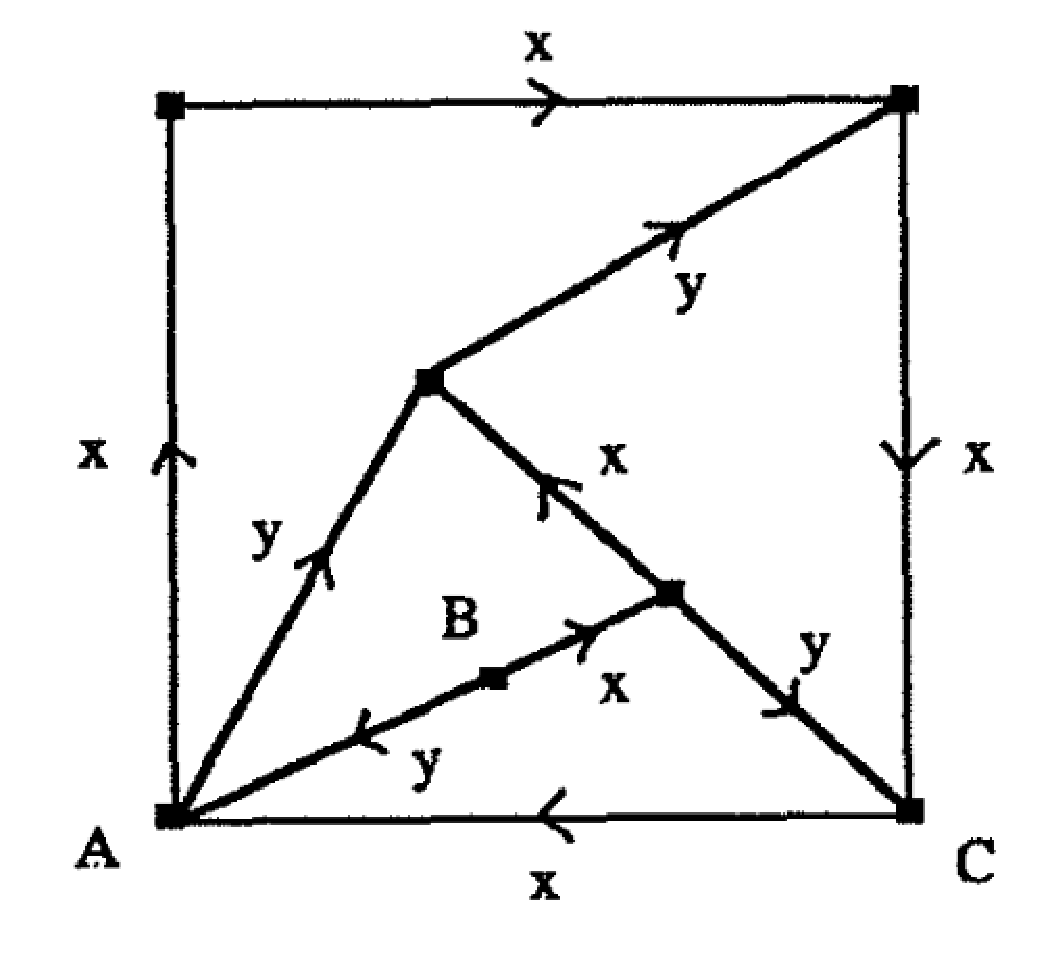
\includegraphics[scale=0.3]{resources/vanKampenDiagram.pdf}
\end{center} Since the boundary label $r = x^4$ can be deduced from the
    internal faces, it follows that \[Q_4 = \Grp{x,y|s=t=1}.\]
\end{eg}

\begin{eg} The group \[F(2,4) = \langle a,b,c,d | ab = c, bc = d, cd = a, da =
    b\rangle\] is generated by $a$ and $b$ since $c = ab$ and $d = bc = bab$.
    We claim that it is actually a cyclic group whose order divides 5
    (therefore is of order 5 or 1). This follows from the following diagrams.
    The faces are labelled by \[r_1 = abc^{-1}, r_2 = bcd^{-1}, r_3 = cda^{-1},
    r_4 = dab^{-1}.\]
\begin{center}
    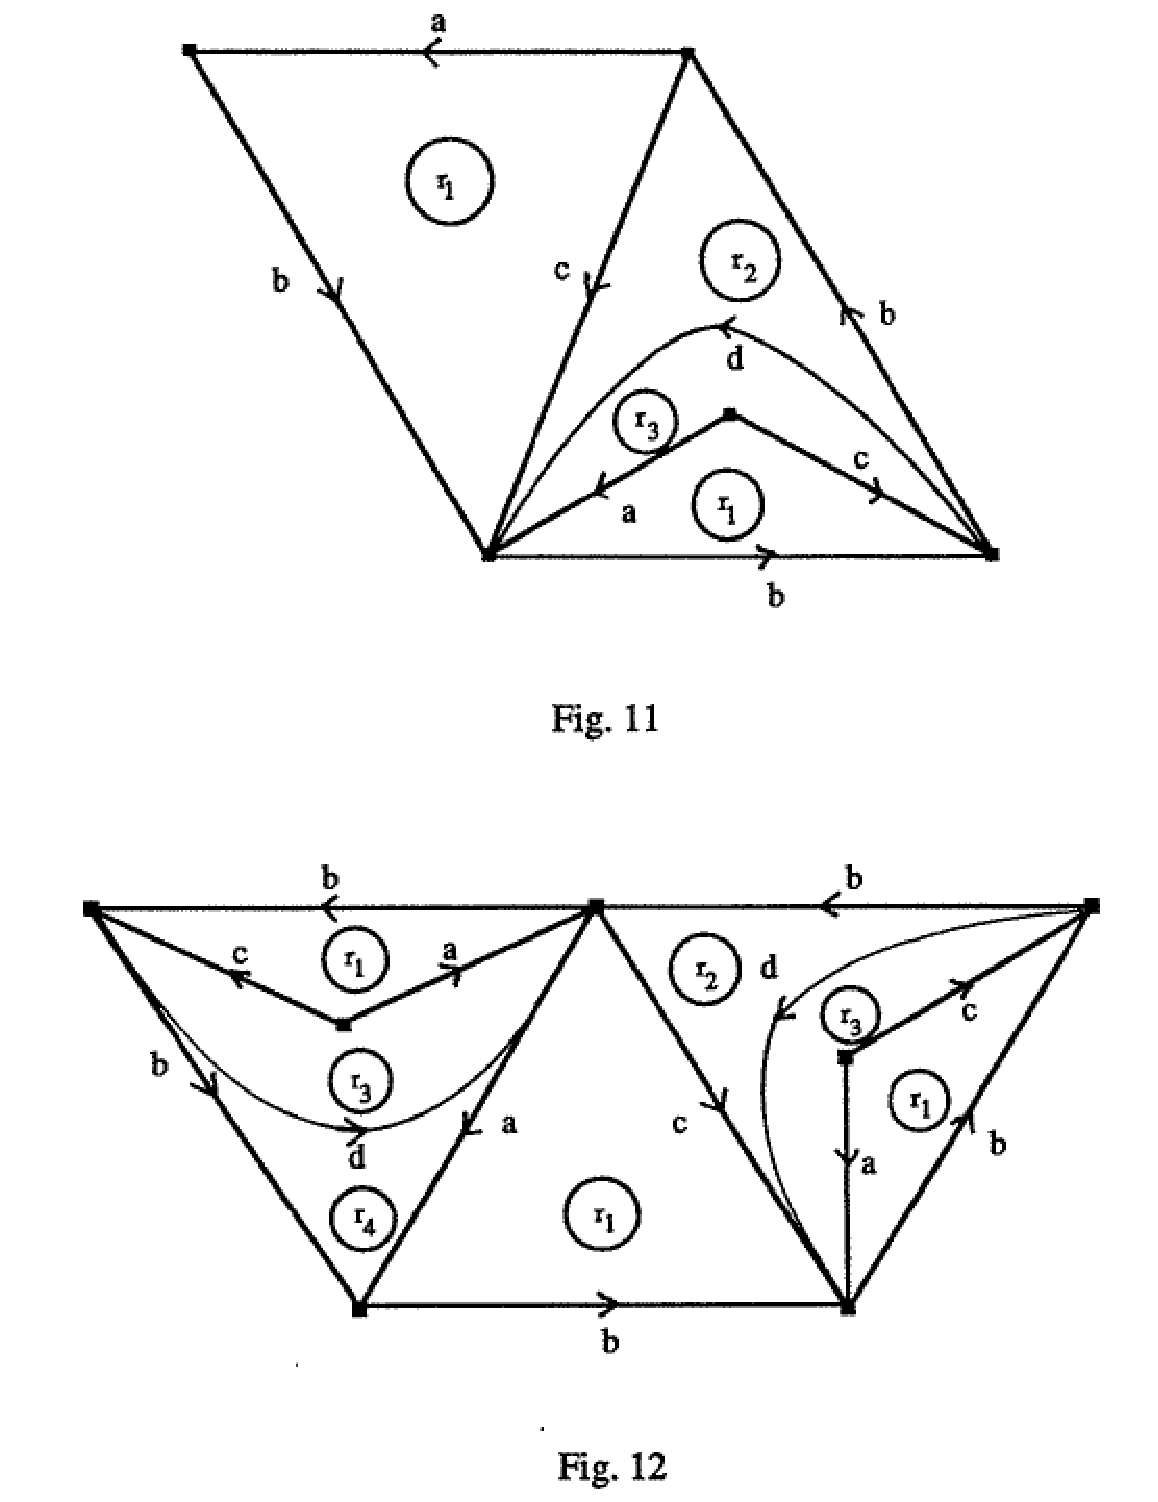
\includegraphics[scale=0.4]{resources/f24.pdf}
\end{center}
    Namely, the first figure shows that $a = b^{-3}$ which implies that the
    group is cyclic and the second shows that $b^5 = 1$ which implies that the
    generator of this cyclic group has order 1 or 5.
\end{eg}

\begin{ap} We will now investigate in detail the generators and relations of
    some important examples of groups. Typically the group $G$ will be given by
    an abstract definition which does not immediately lend itself to the
    determination of a presentation. The method by which we find a presentation
    goes as follows.

    (1) Find a set of generators $X$ of $G$.

    (2) In terms of $X$ find some relations $R=e$ that hold in $G$ and conjecture that these are enough to define $G$.

    (3) Show that the natural surjection (which exists because we know that $X$ generates $G$) \[\pi: \langle X | R \rangle \twoheadrightarrow G \] is an isomorphism.

    It is usually the last step which is the most difficult. For instance, it
    may be possible to bound $|G|$ from below by using properties of an action
    of $G$ on some set and to bound $|\langle X|R\rangle|$ from above by
    looking at the presentation. If these bounds are equal and finite then
    $\pi$ is an isomorphism. More generally, one may find a ``normal form'' for
    the elements of \(\langle X|R\rangle \) i.e.~write down a list $L$ of
    elements of $(X^{\pm})^*$ and then to give a bijection between $L$ and
    \(\langle X|R\rangle\). Let us now look at some examples in detail.
\end{ap}

\begin{rem} Let us make explicit a notational convention which we have already
    used several times without comment. When the context clearly indicates
    whether we are working with groups or with monoids, we will simply write
    \(\langle X |R\rangle\) to mean one of \Mon{X|R} or \Grp{X|R} according to
    the context.
\end{rem}

\begin{eg}[The Quaternions] Let us classify groups of order 8, as follows.
    First, if $G$ is abelian then by the classification of finite abelian
    groups $G \simeq (\Z/2)^{\oplus 3}$ or $\Z/4 \oplus \Z/2$ or $G \simeq
    \Z/8$.

    Suppose that $G$ is nonabelian and let $x\in G$ be an element of maximal
    order $m$. Then $m = 2,4,$ or $8$.

    If $m=2$ then $G$ is abelian ($m=2 \text{ and } a,b\in G \Rightarrow a,b,
    ab$ are all of order 2 $\Rightarrow ba = a^2(ba)b^2 = a(abab)b = a(ab)^2b =
    ab$). If $m=8$ then $G$ is cyclic and therefore abelian. Thus, $G$
    nonabelian $\Rightarrow m=4.$

    Then $H := \langle x\rangle \vartriangleleft G$ since we know that a
    subgroup of index two is normal. Let $y\in G-H$. Then we have that $y^2,
    y^{-1}xy \in H$. It then follows by considering the order of group elements
    that \[y^{-1} x y = x \text{ or } x^{-1} \text{ and } y^2 = e \text{ or }
    x^2. \] (In detail, $y^{-1}xy$ has the same order in $G$ as $x$ thus it
    must be a generator of $H$ since it is in $H$. Regarding $y^2$, if we know
    that it has order dividing $4$ in $H$ but if $y^2 = x \text{ or } x^{-1}$
    then $G$ would be cyclic of order 8 with generator $y$. Therefore $y^2 = e
    \text{ or } x^2.$)

    Now, if $y^{-1}xy = x$ then $G$ is abelian and isomorphic to $\Z/4\oplus
    \Z/2$. If $y^{-1}x y = x^{-1}$ and $y^2 = e$ then $G\simeq D_4$ is a
    dihedral group (we refer you to Dummit and Foote for more details). We are
    reduced the following. Is there a group of order 8 containing an element x
    of order 4 and an element $y\neq x$ with $y^2 = x^2$ and $y^{-1} xy =
    x^{-1}$ There is at most one such group since the information implies that
    all elements of $G$ are of the form \[\{x^i, x^iy : 0 \le i \le 3\}\] and
    the multiplication table is given by
    \[ \begin{array}{c | c | c| }
        & x^j & x^jy \\
        \hline
        x^i & x^{i+j} & x^{i+j}y \\
        \hline
        x^iy & x^{i-j}y & x^{i-j+2} \\
        \hline
    \end{array} \]
    where the powers of $x$ taken with the understanding that $x$ is of order
    4. We must now show that this multiplication table actually defines a
    group. We could check this by hand but let us instead proceed as follows.
    We will construct a group of order 8 which has the above multiplication
    table; the point is that because of the way we will make the construction,
    we can see easily that the cardinality is 8, which is not at all clear from
    the above multiplication table.

    Let \HH{} be the set of matrices in $GL_2(\C)$ of the form \[\left\{
    \begin{pmatrix}
        z & w \\ -\overline{w} & \overline{z}
    \end{pmatrix}
    \right\} \] One checks that if $A,B\in \HH$ then so are $A+B, -A, AB,
    \text{ and } A^{-1}$ (provided that $A\neq 0$ in the last case). Note that
    if $z = a+ib, w =c+id$ are both nonzero then likewise \[\det A =
    z\overline{z} + w\overline{w} = a^2 + b^2 + c^2 + d^2 \neq 0.\] Thus \HH{}
    is a division algebra over \R{} (i.e.~a noncommutative \R-algebra in which
    every nonzero element has a multiplicative inverse), known as the ring of
    quaternions. Writing
    \[I = \begin{pmatrix} 1 & 0 \\ 0 & 1 \end{pmatrix},
    X = \begin{pmatrix} i & 0 \\ 0 -i \end{pmatrix},
    Y = \begin{pmatrix} 0 & 1 \\ -1 & 0 \end{pmatrix},
    Z = \begin{pmatrix} 0 & i \\ i & 0 \end{pmatrix}
    \] then one can see using the coordinates that the elements \[\{\pm I, \pm
    X, \pm Y, \pm Z\}\] are 8 distinct elements of \HH{} and using matrix
    multiplication one can check that this set forms a group $Q_4$ of order 8.
    Finally the relations \[X^4 = I, X^2 = Y^2, Y^{-1}XY = X^{-1}\] all obtain
    in $Q_4$ so that $Q_4$ is isomorphic to the sought group of order 8: \[Q_4
    = \langle x,y | x^4 = e, x^2 = y^2, y^{-1}xy = x^{-1}\rangle.\]
\end{eg}

\begin{eg}[The Symmetric Group] Let \[S_n := \mathrm{Sym}(\{1,2,\dots,n\})\] be
    the symmetric group on $n$ letters. To find a presentation for $S_n$ we
    proceed in three steps.

    (1) Let us first find a generating set. We know that every permutation can
    be written as a product of disjoint cycles so that the cycles generate
    $S_n$.  Since any cycle may be expressed as a product of transposition
    \[(x_1x_2\cdots x_t) = (x_1x_2)(x_1x_3)\cdots(x_1 x_t), \] in fact the
    transpositions generate $S_n$. If $(ij)$ is a transposition with $1 \le
    i<j \le n$ (this accounts for all transpositions since $(ji) = (ij)$) then
    we have \[(ij) = (i\; i+1)(i+1\; i+2) \cdots (j-2\; j-1) (j-1\; j) (j-2\;
    j-1) \cdots (i+1\; i+2)(i\; i+1).\] Therefore $S_n$ is generated by the
    adjacent transpositions \[\{(i\; i+1) : 1 \le i \le n+1\}.\]

    (2) The adjacent transpositions satisfy the following relations:
    \begin{align*}
        (i\; i+1)^2 &= e,& 1 \le i \le n-1,\\
        ( (i\; i+1)(i+1\; i+2) )^3 & = e,& 1 \le i \le n-2,\\
        (i \; i+1)(j\; j+1) & = (j\; j+1)(i\; i+1),& 1 \le i,j \le n-1, |i-j| \ge 2.
    \end{align*}
    Therefore we conjecture that the following is a presentation of $S_n$:
    \[G_n:= \langle x_1, \dots, x_{n-1} | R, S, R\rangle\] where
    \begin{align*}
        R &= \{x_i^2 : 1 \le i \le n-1\}\\
        S &= \{(x_i\; x_{i+1})^3 : 1 \le i \le n-2\},\\
        T &= \{[x_i,x_j] : 1 \le i < j-1 < n-1\}.
    \end{align*} Here, $T$ expresses the fact that disjoint transpositions commute.

    Now, by the above we know that there is a surjection $G_n
    \twoheadrightarrow S_n$ and we must show that it is an isomorphism.

    (3) To show that it is an isomorphism it suffices to show that $|G_n| \le
    n!$. We prove this by induction on $n$. If $n=1$ then $G_1$ is the trivial
    group so there is nothing to prove. Assume now that $n \ge 2$ and that
    $G_{n-1} \le (n-1)!.$ Let $H$ be the subgroup of $G_n$ generated by $x_1,
    \dots, x_{n-2}$ and put \[y_0 := e \text{ and } y_i := x_{n-1}\dots x_{n-i}
    \text{ for } 1 \le i \le n-1. \] Let \[A := \{h y_i : h\in H, 0 \le i \le
    n-1\} \subset G_n.\] We shall show that $A = G_n$. Let us first show that
    \[Ax_j \subset A \text{ for } 1 \le j \le n-1.\] We have to consider the
    terms $hy_ix_j$ in six cases.

    (i) $i = 0, j< n-1 \Rightarrow hy_ix_j = hx_j \in Hy_0 \subset A$

    (ii) $i=0,j=n-1 \Rightarrow hy_i x_j = hex_{n-1} = hy_1 \in Hy_1 \subset A$

    (iii) \begin{align*} i > 0, j > n-i \Rightarrow hy_ix_j &= h(x_{n-1} \cdots x_j x_{j-1} \cdots x_{n-i}) x_j \\
        &= hx_{n-1} \cdots x_j x_{j-1} x_j \cdots x_{n-i} & \text{by } T\\
        &= hx_{n-1} \cdots x_{j-1} x_j x_{j-1} \cdots x_{n-i} & \text{by } R \text{ and } S\\
        &= (hx_{j-1})x_{n-1}\cdots x_{n-i} & \text{by } T\\
        & \in Hy_i \subset A
    \end{align*}

    (iv)
    \begin{align*} i > 0, j=n \Rightarrow hy_i x_j & = hx_{n-1}\cdots x_{n-i}x_{n-i}\\
        &= hx_{n-1}\cdots x_{n-i+1} & \text{by } R\\
        &= hy_{i-1} \in Hy_{i-1} \subset A
    \end{align*}

    (v)
    \begin{align*} i > 0, j < n-i-1 \Rightarrow hy_ix_j &= (hx_j)y_i & \text{by } T\\
        & \in Hy_i \subset A
    \end{align*}

    (vi)
    \begin{align*} i > 0, j < n-i-1 \Rightarrow hy_i x_j &= (hx_j)y_i & \text{by } T \\
        &\in Hy_i \subset A
    \end{align*}

    This shows that $Ax_j \subset A$ for all $j$. Now, by $R$ we have
    \[Ax_j^{-1} = Ax_j \subset A \text{ for } 1 \le j \le n-1.\]

    Thus there is an injection from $G_n$ to $A$, i.e.~$A$ consists of the
    elements of $G_n$ written in ``normal form'' with respect to the subgroup
    $G_{n-1}$. Since the relations in $G_{n}$ which involve $x_1,\dots,x_{n-2}$
    are exactly those from $G_{n-1}$ it follows that the map $\varphi : G_{n-1}
    \rightarrow G_n$ given by $x_i \mapsto x_i$ is a group homomorphism. Since
    $\Im \varphi = H$ (by definition) and $|G_{n-1} \le (n-1)!$ by the
    induction hypothesis, it follows that \[|G_n| \le |A| \le n|H| \le n!\] as
    required.
\end{eg}

